%!TEX root = ./main.tex
%
% This file is part of the i10 thesis template developed and used by the
% Media Computing Group at RWTH Aachen University.
% The current version of this template can be obtained at
% <http://www.media.informatik.rwth-aachen.de/karrer.html>.

\documentclass[11pt, a4paper, titlepage]{book}
\usepackage[ngerman]{babel}
\usepackage{pdfpages}   % This is your set screw

% ! ACHTUNG !
% Nach dem ersten LaTeX durchlauf auf der Kommandozeile
% makeindex -s main.ist main.idx
% ausf�hren, sonst wird der Index nicht so sch�n formatiert.
% Leider macht TeXShop den makeindex Aufruf nur ohne Parameter.

% !ATTENTION!
% After running LaTeX for the first time using this template call
% makeindex -s main.ist main.idx
% to get the correct formatting for the index.

%Pakete und eigene Befehle - am besten durchlesen!
%Includes all neccessary packets and contains some useful commands - read this file!
%!TEX root = ./main.tex

% This file is part of the i10 thesis template developed and used by the
% Media Computing Group at RWTH Aachen University.
% The current version of this template can be obtained at
% <http://www.media.informatik.rwth-aachen.de/karrer.html>.



%-----------------------------------------------------------------------------------------------------------------------------------------
% Befehle
% commands
%-----------------------------------------------------------------------------------------------------------------------------------------

%----------------------------------------------------------------------------------
% \myBigFigure	[ LABEL_PREFIX (optional) ]
%				{ FILENAME (without extension) }
%				{ CAPTION TEXT }
%				{ SHORT VERSION OF CAPTION TEXT }
%
%Bild wird in kompletter Breite gesetzt, die Kurzversion der Bildunterschrift erscheint im Abbildungsverzeichnis
%picture using full width of the page, the short caption is what appears in the list of figures index

%----------------------------------------------------------------------------------
% \myFrameBigFigure	[ LABEL_PREFIX (optional) ]
%					{ FILENAME (without extension) }
%					{ CAPTION TEXT }
%					{ SHORT VERSION OF CAPTION TEXT }
%
%Bild wird in kompletter Breite gesetzt und eingerahmt, die Kurzversion der Bildunterschrift erscheint im Abbildungsverzeichnis
%picture with frame using the full width of the page, the short caption is what appears in the list of figures index

%----------------------------------------------------------------------------------
% \myHUGEFigure	[ LABEL_PREFIX (optional) ]
%				{ FILENAME (without extension) }
%				{ CAPTION TEXT }
%				{ SHORT VERSION OF CAPTION TEXT }
%
%Bild wird rotiert und quer in kompletter Breite gesetzt, die Kurzversion der Bildunterschrift erscheint im Abbildungsverzeichnis
%landscape picture using the full width of the rotated page, the short caption is what appears in the list of figures index

%----------------------------------------------------------------------------------
% \myFigure	[ LABEL_PREFIX (optional) ]
%			{ FILENAME (without extension) }
%			{ CAPTION TEXT }
%			{ SHORT VERSION OF CAPTION TEXT }
%
%Bild wird in der Breite der textspalte gesetzt, die Kurzversion der Bildunterschrift erscheint im Abbildungsverzeichnis
%picture using the width of the text column, the short caption is what appears in the list of figures index

%----------------------------------------------------------------------------------
% \myImgRef	[ LABEL_PREFIX (optional) ]
%			{ LABEL OF THE IMAGE }
%
%referenziert das angegebene Bild
%reference to an image

%----------------------------------------------------------------------------------
% \myBigTable	{ YOUR TABULAR DEFINITION }
%			{ CAPTION TEXT }
%			{ TABLE_LABLE }
%
%Tabelle wird in kompletter Breite gesetzt
%table using the full width of the page

%----------------------------------------------------------------------------------
% \myTable	{ YOUR TABULAR DEFINITION }
%			{ CAPTION TEXT }
%			{ TABLE_LABLE }
%
%Tabelle wird in der Breite der Textspalte gesetzt
%table using the width of the text column

%----------------------------------------------------------------------------------
% \myTxtRef	{ LABLE }
%
%Referenz auf Kapitel oder Abschnitte - gibt nummer und namen aus, z.B.: 5.3---"Yaddahyaddah"
%references chapters or sections, outputs number and title, e.g., 5.3---"Yaddahyaddah"

%----------------------------------------------------------------------------------
% \myUnderscore
%
%Setzt einen "sch�nen" Unterstrich f�r URLs
%typesets a 'nice' underscore for URLs

%----------------------------------------------------------------------------------
%\myTilde
%
%Setzt eine "sch�ne" Tilde f�r URLs
%typesets a 'nice' tilde for URLs

%----------------------------------------------------------------------------------
% \myURL	{ TYPESET VERSION OF ANCHOR }
%			{ PRISTINE URL }
%			{ TYPESET VERSION OF URL }
%
%Setzt eine URL
%die typographisch "sch�ne" version erscheint in einer Fu�note,
%im Text erscheint der Ankertext, verlinkt ist die "echte" URL
%typesets a URL
%the typographically correct version appears as a footnote,
%the anchor appears in the text, the link points to the pristine URL

%----------------------------------------------------------------------------------
% \mySimpleURL	{ TYPESET VERSION OF ANCHOR }
%				{ PRISTINE URL }
%
%Setzt eine URL
%die URL erscheint in einer Fu�note,
%im Text erscheint der Ankertext, die URL ist verlinkt
%typesets a URL
%the URL appears as a footnote,
%the anchor appears in the text, the link points to the URL

%----------------------------------------------------------------------------------
% \myProjectURL	{ TYPESET VERSION OF ANCHOR }
%				{ PRISTINE URL INSIDE PROJECT DIRECTORY }
%				{ TYPESET VERSION OF URL INSIDE PROJECT DIRECTORY }
%
%Setzt eine URL innerhalb des Projektverzeichnisses auf "media"
%ACCOUNT muss durch den eigenen Usernamen ersetzt werden
%die typographisch "sch�ne" version erscheint in einer Fu�note,
%im Text erscheint der Ankertext, verlinkt ist die "echte" URL
%typesets a URL inside the project directory on 'media'
%replace ACCOUNT with your username
%the typographically correct version appears as a footnote,
%the anchor appears in the text, the link points to the pristine URL

%----------------------------------------------------------------------------------
% \mnote	{ MARGIN NOTE }
%
%Setzt eine Randnotitz
%puts a comment into the margin in small sans-serif font

%----------------------------------------------------------------------------------
% \todo	{ TODO MARGIN NOTE }
%
%Setzt eine "ToDo"-Randnotitz in rot zur Erinnerung
%puts a 'todo' comment into the margin in red

%----------------------------------------------------------------------------------
% \chapterquote	{ QUOTATION }
%				{ SOURCE }
%
%Setzt ein Zitat zum Einleiten eines Kapitels
%outputs a quote with its source, can be used as an introduction to chapters

%----------------------------------------------------------------------------------
% \myDefBox	{ TERM }
%			{ DEFINITION }
%
%Setzt eine Randnotitz und eine farbige Box (Textspaltenbreite),
%welche einen Begriff und seine Definition enth�lt
%outputs a margin note and a colored box (width of the text column) containing a term and its definition

%----------------------------------------------------------------------------------
% \myBigDefBox	{ TERM }
%				{ DEFINITION }
%
%Setzt eine farbige Box (Seitenbreite), welche einen Begriff und seine Definition enth�lt
%outputs a colored box (width of the page) containing a term and its definition

%----------------------------------------------------------------------------------
% \myDownloadURL	{ TYPESET DOWNLOAD NAME }
%					{ PRISTINE VERSION OF FILENAME }
%					{ TYPESET VERSION OF FILENAME }
%
%Setzt eine farbige Box, welche einen Downloadlink enth�lt
%outputs a colored box containing a download link

%----------------------------------------------------------------------------------
% \emptydoublepage
%
% Leere Doppelseite ohne Kopf- oder Fu�zeile am Ende von Kapiteln
% Clear double page without any header or footer at end of chapters

%----------------------------------------------------------------------------------
% \pagebreak	[ SOME STRANGE LATEX VALUE ]
%
%Eklige pagebreaks f�r den Druck (falls es nicht mehr anders geht)
%pagebreaks for the final print version (last resort weapon against wrong pagebreaks by LaTeX)

%----------------------------------------------------------------------------------
% \TM
%
%Setzt ein (TM) Symbol
%Places a (TM) symbol


%----------------------------------------------------------------------------------
%Packages and parameters
%----------------------------------------------------------------------------------

%Inputencoding f�r den Mac
%inputencoding for the mac
\usepackage[utf8]{inputenc}

%Mathe- und Symbolpakete
%packages for mathematical symbols
\usepackage{latexsym}
\usepackage{amsmath}
\usepackage{amssymb}

%Tabellengestaltung
%table design
\usepackage{booktabs}

%Grafikpaket
%grahics package
\usepackage{color,graphicx}
\usepackage{caption}
\usepackage{subcaption}

%relativer Pfad zu den Bildern
%path to your image folder
\graphicspath{{images/}}

%Abs�tze werden nicht eingezogen, sondern vertikal abgesetzt
%do not indent at new paragraphs but add a vertical offset
\usepackage{noindent}

%Palatino+Helvetica statt Computer Modern als standard fonts:
%change standard fonts to Palatino and Helvetica
\usepackage{palatino}

%Bibliographieeinstellungen
%bibliography settings
\usepackage{natbib}
%\bibliographystyle{plainnat}


%Zitierbefehle
%citation commands
\newcommand{\fullcite}{\citep} %for "Author [1980]"
\renewcommand{\citeyear}{\citeyearpar} %for "[1980]"

%paket f�r erweiterte kontrollstrukturen
%package for control structures
\usepackage{ifthen}

%marginpar hack --- alle Randnotitzen sollten dann auf der richtigen Seite stehen
%marginpar hack --- moves margin notes to correct position
\usepackage{mparhack}

%lesbare verweise
%make readable references
\usepackage[plainpages=false,pdfpagelabels,bookmarks=true]{hyperref}

%bookmark in pdf
\usepackage{bookmark}

%--------------------------------------------------------------------------------------------------
%Justify without hyphenation
%https://sumanta679.wordpress.com/2009/05/20/latex-justify-without-hyphenation/
\tolerance=1
\emergencystretch=\maxdimen
\hyphenpenalty=10000
\hbadness=10000
%--------------------------------------------------------------------------------------------------

%---------------------<Layout in the style of "A Pattern Approach to Interaction Design>---------------------------

% Change page headers and footers:
\usepackage{fancyhdr}
%inserting text files
\usepackage{listings}
\usepackage{color}
\usepackage{fancyvrb}
\usepackage{alltt}
\usepackage{verbatim}
\usepackage{verbatimbox}
\usepackage{fancyvrb}
\usepackage{sverb}
\usepackage{graphicx}       % logo
\usepackage[export]{adjustbox}  % align logo to the top right side page


%New colors defined below
\definecolor{codegreen}{rgb}{0,0.6,0}
\definecolor{codegray}{rgb}{0.5,0.5,0.5}
\definecolor{codepurple}{rgb}{0.58,0,0.82}
\definecolor{backcolour}{rgb}{0.95,0.95,0.92}

%Code listing style named "mystyle"
\lstdefinestyle{mystyle}{
  backgroundcolor=\color{backcolour},   commentstyle=\color{codegreen},
  keywordstyle=\color{magenta},
  numberstyle=\tiny\color{codegray},
  stringstyle=\color{codepurple},
  basicstyle=\footnotesize,
  breakatwhitespace=false,         
  breaklines=true,                 
  captionpos=b,                    
  keepspaces=true,                 
  numbers=left,                    
  numbersep=5pt,                  
  showspaces=false,                
  showstringspaces=false,
  showtabs=false,                  
  tabsize=2
}

%"mystyle" code listing set
\lstset{style=mystyle}

\pagestyle{fancy}
\fancyhf{}
%\fancyhead[RE]{\slshape \nouppercase{\leftmark}}    % Even page header: "page   chapter"
%\fancyhead[LO]{\slshape \nouppercase{\rightmark}}   % Odd  page header: "section   page"
%\fancyhead[RO,LE]{\bfseries \thepage} 
\renewcommand{\headrulewidth}{1pt}    % Underline headers
\renewcommand{\footrulewidth}{0pt}

\fancyhead[R]{\bfseries\thepage}
%\fancyhead[L]{
\includegraphics[width = 50mm, left]{images/rwth_sm_leichtbau_schwarz_grau_rgb}}

\fancypagestyle{plain}{               % No chapter+section on chapter start pages
\fancyhf{}
%\fancyhead[RO,LE]{\bfseries \thepage}
\fancyhead[R]{\bfseries\thepage}
%\fancyhead[L]{
\includegraphics[width = 50mm, left]{images/rwth_sm_leichtbau_schwarz_grau_rgb}}
\renewcommand{\headrulewidth}{1pt}
\renewcommand{\footrulewidth}{0pt}
}

% Left headings: "1  INTRODUCTION"
\renewcommand{\chaptermark}[1]{%
\markboth{\thechapter\ \ \ \ #1}{}}

% Right headings: "1.1  Basics"
\renewcommand{\sectionmark}[1]{%
\markright{\thesection\ \ \ \ #1}{}}

% some Fancyhdr problem...
\addtolength{\headheight}{2pt} % To avoid overfull vboxes from fancyhdr


%creating a better way to change the layout for the abstract pages
\usepackage[head=50pt]{geometry}

%decrease the vertical space between the top of the page and the chapter heading
\usepackage{titlesec}
\makeatletter
\def\@makeschapterhead#1{%
  %%%%%\vspace*{50\p@}% %%% removed!
  {\parindent \z@ \raggedright
    \normalfont
    \interlinepenalty\@M
    \Huge \bfseries  #1\par\nobreak
    \vskip 20\p@
  }}
\makeatother

\ifthenelse{\lengthtest{\paperheight=250mm}}%
{% -----------------B5 Layout-----------------
% Page layout

%\pdfpageheight250mm
%\pdfpagewidth176mm
\geometry{	b5paper,
			top = 27mm, %27mm
			footskip = 10mm,
			inner = 19mm,
			outer = 39mm,
			textheight = 175mm,
			textwidth = 84mm,
			marginparsep = 0mm, %3mm
			marginparwidth = 0mm %32mm
}
\savegeometry{myText}
% -----------------/ B5 Layout-----------------
}%
{% -----------------A4 Layout-----------------
% Page layout
\geometry{	a4paper,
			twoside,
			includemp,
			includehead,
			top = 20mm, %30mm
			headsep = 10mm, %10mm
			bindingoffset = 10mm, %10mm
			inner = 20mm, %20mm
			outer = 30mm, %40mm
			bottom = 30mm, %45mm
			marginparsep = 0mm, %10mm
			marginparwidth = 0mm %30mm
}
\savegeometry{myText}
% -----------------/ A4 Layout-----------------
}
% Abstract layout
\geometry{	marginparsep = 0mm,
			marginparwidth = 0mm
}
\savegeometry{myAbstract}
\loadgeometry{myText}


\newlength{\fullwidth} % Width of text plus margin notes
\setlength{\fullwidth}{\textwidth}
\addtolength{\fullwidth}{\marginparsep}
\addtolength{\fullwidth}{\marginparwidth}

\setlength{\headwidth}{\fullwidth} % Header stretches over margin notes


%---------------------</Layout in the style of "A Pattern Approach to Interaction Design>---------------------------


%wird f�r die fl�chendeckende Ausgabe der Titelseite ben�tigt
%needed for the full-face titlepage
\usepackage{eso-pic}


%index verwenden
%make an index
\usepackage[nonewpage]{imakeidx}
 %below multiple columns wont work, if there is \renewenvironment{theindex} afterwards
\makeindex[columns=2]

%Index Formatierungshilfen
%formatting helpers for the index
\newcommand{\uu}[1]{\underline{#1}}
\newcommand{\ii}[1]{\textit{#1}}

%neue Definition der Index Umgebung
%redesign of the index
\iffalse
\renewenvironment{theindex}{%
  \vspace*{50pt}%
  {\Huge\bfseries\indexname}\par%
  \vspace*{40pt}%
  \setlength{\parskip}{0pt}%
  \setlength{\parindent}{0pt}%
  \small%
  \renewcommand{\item}{\par{}}%
  \renewcommand{\subitem}{\par\hspace{2em}- }%
}%
{}
\fi

%Maximale Gliederungstiefe, die noch ins Inhaltsverzeichnis aufgenommen wird
%maximum depth for the table of contents
\setcounter{tocdepth}{3}

%Vorschlag f�r ein sch�nes Farbschema
%Set of colors which look nice together
\usepackage{color}
\definecolor{orange_light}{rgb}{1,0.8,0.4}
\definecolor{orange_med}{rgb}{0.753,0.62,0.373}
\definecolor{orange_dark}{rgb}{0.506,0.412,0.251}

\definecolor{green_light}{rgb}{0.8,1,0.4}
\definecolor{green_med}{rgb}{0.635,0.745,0.376}
\definecolor{green_dark}{rgb}{0.435,0.498,0.255}

\definecolor{blue_light}{rgb}{0.4,0.8,1}
\definecolor{blue_med}{rgb}{0.365,0.624,0.749}
\definecolor{blue_dark}{rgb}{0.251,0.42,0.502}

\definecolor{pink_light}{rgb}{1,0.435,0.812}
\definecolor{pink_med}{rgb}{0.745,0.38,0.62}
\definecolor{pink_dark}{rgb}{0.498,0.255,0.416}

\definecolor{yellow_light}{rgb}{1,1,0.4}
\definecolor{yellow_med}{rgb}{0.757,0.745,0.373}
\definecolor{yellow_dark}{rgb}{0.506,0.49,0.251}

%blau (f�r URLs)
%blue (for URLs)
\definecolor{blue}{rgb}{0,0,1}

%notwendig f�r die korrekte Erkennung, auf welcher Seite sich eine Abbildung befindet.
%we need this to determine if a figure is on an odd or even page
\usepackage{chngpage}

%Hiermit k�nnen die Abbildungslegenden frei gestaltet werden
%we need this to redesign the captions
\usepackage[font=normalsize,labelfont=bf]{caption}

%Abbildungen kommen auf eine eigene Seite, wenn sie mehr als 85% des Platzes
%auf einer Seite einnehmen
%if a figure takes more than 85% of a page it will be typeset on a separate page
\renewcommand{\floatpagefraction}{0.85}

%Ben�tigt um gro�e Abbildungen gedreht auf eine Seite zu setzen
%we need this to rotate big figures
\usepackage[figuresright]{rotating}

%Verschiedene L�ngenma�e f�r Textboxen
%dimensions for textboxes
\newlength{\myDefBoxWidth}
\setlength{\myDefBoxWidth}{\textwidth}
\addtolength{\myDefBoxWidth}{-4mm}
\newlength{\myBigDefBoxWidth}
\setlength{\myBigDefBoxWidth}{\fullwidth}
\addtolength{\myBigDefBoxWidth}{-4mm}

%Formathilfen f�r MatLab Code (wer's braucht...)
%pre-defined matlab code formats
\usepackage{alltt}
\definecolor{string}{rgb}{0.7,0.0,0.0}
\definecolor{comment}{rgb}{0.13,0.54,0.13}
\definecolor{keyword}{rgb}{0.0,0.0,1.0}



%-----------------------------------------------------------------------------------------------------------------------------------------
% neue Befehle
% new commands
%-----------------------------------------------------------------------------------------------------------------------------------------

%----------------------------------------------------------------------------------
% \myBigFigure	[ LABEL_PREFIX (optional) ]
%				{ FILENAME (without extension) }
%				{ CAPTION TEXT }
%				{ SHORT VERSION OF CAPTION TEXT }
%
%Bild wird in kompletter Breite gesetzt
%picture using full width of the page
\newcommand{\myBigFigure}[4][image]
{%
\begin{figure}[t!bp]%
	\checkoddpage%
	\ifcpoddpage%
		%nothing
	\else
		\hspace{-\marginparsep}\hspace{-\marginparwidth}%
	\fi
	%use minipage to center the label beneath the figure
	\begin{minipage}{\fullwidth}%
		\includegraphics[width= \fullwidth]{#2}%
		\caption[#4]{#3}%
		\label{#1_#2}%
	\end{minipage}%
\end{figure}%
}


%----------------------------------------------------------------------------------
% \myFrameBigFigure	[ LABEL_PREFIX (optional) ]
%					{ FILENAME (without extension) }
%					{ CAPTION TEXT }
%					{ SHORT VERSION OF CAPTION TEXT }
%
%Bild wird in kompletter Breite gesetzt und eingerahmt
%picture with frame using the full width of the page
\newcommand{\myFrameBigFigure}[4][image]
{
\begin{figure}[t!bp]
	\checkoddpage
	\ifcpoddpage
		%nothing
	\else
		\hspace{-\marginparsep}\hspace{-\marginparwidth}
	\fi
	%use minipage to center the label beneath the figure
	\begin{minipage}{\fullwidth}
	\frame{%
		\includegraphics[width= \fullwidth]{#2}%
		}
		\caption[#4]{#3}
		\label{#1_#2}
	\end{minipage}
\end{figure}
}

%----------------------------------------------------------------------------------
% \myHUGEFigure	[ LABEL_PREFIX (optional) ]
%				{ FILENAME (without extension) }
%				{ CAPTION TEXT }
%				{ SHORT VERSION OF CAPTION TEXT }
%
%Bild wird rotiert und quer in kompletter Breite gesetzt
%landscape picture using the full width of the rotated page
\newcommand{\myHugeFigure}[4][image]
{
\begin{sidewaysfigure}[t!bp]
	\checkoddpage
	\ifcpoddpage
		%nothing
		\vspace{\marginparsep}\vspace{\marginparwidth}
	\else
		%nothing
		\vspace{-\marginparsep}\vspace{-\marginparwidth}
	\fi
		\includegraphics[width= \textheight]{#2}
		\caption[#4]{#3}
		\label{#1_#2}
	
\end{sidewaysfigure}
}

%----------------------------------------------------------------------------------
% \myFigure	[ LABEL_PREFIX (optional) ]
%			{ FILENAME (without extension) }
%			{ CAPTION TEXT }
%			{ SHORT VERSION OF CAPTION TEXT }
%
%Bild wird in der Breite der textspalte gesetzt
%picture using the width of the text column
\newcommand{\myFigure}[4][image]%
{%
\begin{figure}[t!bp]%
	\begin{center}%
		\includegraphics[width= \textwidth]{#2}%
		\caption[#4]{#3}
		\label{#1_#2}%
	\end{center}%
\end{figure}%
}%

%----------------------------------------------------------------------------------
% \myImgRef	[ LABEL_PREFIX (optional) ]
%			{ LABEL OF THE IMAGE }
%
%referenziert das angegebene Bild
%reference to an image
\newcommand{\myImgRef}[2][image]%
{%
	\ref{#1_#2}%
}%

%----------------------------------------------------------------------------------
% \myBigTable	{ YOUR TABULAR DEFINITION }
%			{ CAPTION TEXT }
%			{ TABLE_LABLE }
%
%Tabelle wird in kompletter Breite gesetzt
%table using the full width of the page
\newcommand{\myBigTable}[3]%
{%
\begin{table}[htdp]%
	\checkoddpage%
	\ifcpoddpage%
		%nothing
	\else%
		\hspace{-\marginparsep}\hspace{-\marginparwidth}%
	\fi%
	\begin{minipage}{\fullwidth}%
		\begin{center}%
			#1%
			\caption{#2}%
			\label{#3}%
		\end{center}%	
	\end{minipage}%
\end{table}%
}%

%----------------------------------------------------------------------------------
% \myTable	{ YOUR TABULAR DEFINITION }
%			{ CAPTION TEXT }
%			{ TABLE_LABLE }
%
%Tabelle wird in der Breite der Textspalte gesetzt
%table using the width of the text column
\newcommand{\myTable}[3]%
{%
\begin{table}[htdp]%
	\begin{center}%
		#1%
		\caption{#2}%
		\label{#3}%
	\end{center}%	
\end{table}%
}%

%----------------------------------------------------------------------------------
% \myTxtRef	{ LABLE }
%
%Referenz auf Kapitel oder Abschnitte - gibt nummer und namen aus, z.B.: 5.3---"Yaddahyaddah"
%references chapters or sections, outputs number and title, e.g., 5.3---"Yaddahyaddah"
\newcommand{\myTxtRef}[1]
{%
	\ref{#1} ``\nameref{#1}''%
}

%----------------------------------------------------------------------------------
% \myTxtRefPP	{ LABLE }
%
%Referenz auf Kapitel oder Abschnitte - gibt nummer, namen und seiten aus, z.B.: 5.3---"Yaddahyaddah" (p. 45)
%references chapters or sections, outputs number and title, e.g., 5.3---"Yaddahyaddah"
\newcommand{\myTxtRefPP}[1]
{%
	\ref{#1} ``\nameref{#1}'' (p.~\pageref{#1})%
}

%----------------------------------------------------------------------------------
% \myUnderscore
%
%Setzt einen "sch�nen" Unterstrich f�r URLs
%typesets a 'nice' underscore for URLs
\newcommand{\myUnderscore}{$\underline{\hspace{0.5em}}$}

%----------------------------------------------------------------------------------
%\myTilde
%
%Setzt eine "sch�ne" Tilde f�r URLs
%typesets a 'nice' tilde for URLs
\newcommand{\myTilde}{$\sim$}

%----------------------------------------------------------------------------------
% \myURL	{ TYPESET VERSION OF ANCHOR }
%			{ PRISTINE URL }
%			{ TYPESET VERSION OF URL }
%
%Setzt eine URL
%die typographisch "sch�ne" version erscheint in einer Fu�note,
%im Text erscheint der Ankertext, verlinkt ist die "echte" URL
%typesets a URL
%the typographically correct version appears as a footnote,
%the anchor appears in the text, the link points to the pristine URL
\newcommand{\myURL}[3]%
{%
	\textcolor{blue}{%
		\href{#2}{#1}%
	}%
	\footnote{#3}%
}

%----------------------------------------------------------------------------------
% \mySimpleURL	{ TYPESET VERSION OF ANCHOR }
%				{ PRISTINE URL }
%
%Setzt eine URL
%die URL erscheint in einer Fu�note,
%im Text erscheint der Ankertext, die URL ist verlinkt
%typesets a URL
%the URL appears as a footnote,
%the anchor appears in the text, the link points to the URL
\newcommand{\mySimpleURL}[2]%
{%
	\textcolor{blue}{%
		\href{#2}{#1}%
	}%
	\footnote{#2}%
}

%----------------------------------------------------------------------------------
% \myProjectURL	{ TYPESET VERSION OF ANCHOR }
%				{ PRISTINE URL INSIDE PROJECT DIRECTORY }
%				{ TYPESET VERSION OF URL INSIDE PROJECT DIRECTORY }
%
%Setzt eine URL auf hci/public wo die Inhalte des WebServer Ordners auf "oliver" verf�gbar sind
%die typographisch "sch�ne" version erscheint in einer Fu�note,
%im Text erscheint der Ankertext, verlinkt ist die "echte" URL
%typesets a URL to hci/public from where the contents of the WebServer folder from oliver can be accessed
%the typographically correct version appears as a footnote,
%the anchor appears in the text, the link points to the pristine URL
\newcommand{\myProjectURL}[3]%
{%
	\textcolor{blue}{%
		\href{http://hci.rwth-aachen.de/public/#2}{#1}%
	}%
	\footnote{http://hci.rwth-aachen.de/public/#3}%
}

%----------------------------------------------------------------------------------
% \mnote	{ MARGIN NOTE }
%
%Setzt eine Randnotitz
%puts a comment into the margin in small sans-serif font
\newcommand{\mnote}[1]%
{%
	\leavevmode%
	\checkoddpage%
	\ifcpoddpage%
		\marginpar{\raggedright\textsf{{\footnotesize{#1}}}}%
	\else%
		\marginpar{\raggedleft\textsf{{\footnotesize{#1}}}}%
	\fi%
}
	
% leavevmode allows mnotes to be aligned with the first line of a paragraph
% NOTE: you have to put a "%" at the end of the line with the mnote, or you will get an extra blank at the beginning of the paragraph!

%----------------------------------------------------------------------------------
% \todo	{ TODO MARGIN NOTE }
%
%Setzt eine "ToDo"-Randnotitz in rot zur Erinnerung
%puts a 'todo' comment into the margin in red
\definecolor{red}{rgb}{1,0,0}
\newcommand{\todo}[1]{\mnote{\textcolor{red}{ToDo: #1}}}

%----------------------------------------------------------------------------------
% \chapterquote	{ QUOTATION }
%				{ SOURCE }
%
%Setzt ein Zitat zum Einleiten eines Kapitels
%outputs a quote with its source, can be used as an introduction to chapters
\newcommand{\chapterquote}[2]{
\begin{quotation}
    \begin{flushright}
	\noindent\emph{``{#1}''\\[1.5ex]---{#2}}
    \end{flushright}
\end{quotation}
}

%----------------------------------------------------------------------------------
% \myDefBox	{ TERM }
%			{ DEFINITION }
%
%Setzt eine Randnotitz und eine farbige Box (Textspaltenbreite),
%welche einen Begriff und seine Definition enth�lt
%outputs a margin note and a colored box (width of the text column) containing a term and its definition
\newcommand{\myDefBox}[2]
{%
	\setlength{\fboxrule}{1mm}%
	\fcolorbox{orange_med}{orange_light}%
	{%
		\parbox{\myDefBoxWidth}{{\bfseries\scshape#1:}\\#2}%
	}%
	\mnote{Definition:\\\emph{#1}}
}

%----------------------------------------------------------------------------------
% \myBigDefBox	{ TERM }
%				{ DEFINITION }
%
%Setzt eine farbige Box (Seitenbreite), welche einen Begriff und seine Definition enth�lt
%outputs a colored box (width of the page) containing a term and its definition
\newcommand{\myBigDefBox}[2]
{%
	\begin{figure}[h!]
	\setlength{\fboxrule}{1mm}%
	\checkoddpage%
	\ifcpoddpage%
		%nothing
	\else%
		\hspace{-\marginparsep}\hspace{-\marginparwidth}%
	\fi%
	\fcolorbox{orange_med}{orange_light}%
	{%
		\parbox{\myBigDefBoxWidth}{{\bfseries\scshape#1:}\\#2}%
	}%
	\end{figure}
}

%----------------------------------------------------------------------------------
% \myDownloadURL	{ TYPESET DOWNLOAD NAME }
%					{ PRISTINE VERSION OF FILENAME }
%					{ TYPESET VERSION OF FILENAME }
%
%Setzt eine farbige Box, welche einen Downloadlink enth�lt
%outputs a colored box containing a download link
\newcommand{\myDownloadURL}[3]{%
\checkoddpage%
	\ifcpoddpage%
		%nothing
	\else%
		\hspace{-\marginparsep}\hspace{-\marginparwidth}%
	\fi%
\setlength{\fboxrule}{1mm}%
\fcolorbox{green_med}{green_light}{%
\begin{minipage}{\myBigDefBoxWidth}%
\begin{center}%
\myProjectURL{#1}{folder/#2}{folder/#3}%
\end{center}%
\end{minipage}%
}%
}

%----------------------------------------------------------------------------------
% \emptydoublepage
%
% Leere Doppelseite ohne Kopf- oder Fu�zeile am Ende von Kapiteln
% Clear double page without any header or footer at end of chapters
\newcommand{\emptydoublepage}{\clearpage\thispagestyle{empty}\cleardoublepage}

%----------------------------------------------------------------------------------
% \pagebreak	[ SOME STRANGE LATEX VALUE ]
%
%Eklige pagebreaks f�r den Druck (falls es nicht mehr anders geht)
%pagebreaks for the final print version (last resort weapon against wrong pagebreaks by LaTeX)
\newcommand{\PB}[1][3]
{%
	\pagebreak[#1]%
}



%----------------------------------------------------------------------------------
% \TM
%
%Setzt ein (TM) Symbol
%Places a (TM) symbol
\newcommand{\TM}
{%
	\textsuperscript{\texttrademark}%
}



%--------------------------------------------------------------
%Dokumentspezifisches
%Stuff regarding your specific document
%--------------------------------------------------------------

%Trennungshilfen
%Hyphenation patterns
\hyphenation{
dieseswortwirdnichtgetrennt
diesesauchnicht
thiswordwillstayinoneline
thistoo
}
%--------------------------------------------------------------
% for making node trees
\usepackage{tikz}
\usetikzlibrary{arrows}

\tikzset{
  treenode/.style = {align=center, inner sep=0pt, text centered,
    font=\sffamily},
  arn_n/.style = {treenode, circle, white, font=\sffamily\bfseries, draw=black,
    fill=black, text width=1.5em},% arbre rouge noir, noeud noir
  arn_r/.style = {treenode, circle, red, draw=red, 
    text width=1.5em, very thick},% arbre rouge noir, noeud rouge
  arn_x/.style = {treenode, rectangle, draw=black,
    minimum width=0.5em, minimum height=0.5em}% arbre rouge noir, nil
}

%--------------------------------------------------------------
\usepackage{float}
%--------------------------------------------------------------
% for structogramms
\usepackage[pict2e,german]{struktex}
%--------------------------------------------------------------
\begin{document}

% gr��ere Wortabst�nde zulassen, um Trennungen zu vermeiden
% allow more flexible whitespaces to avoid hyphenation and overfull hboxes
\sloppy

% "see" Eintr�ge f�r den Index
% 'see'-entries for the index
%!TEX root = ./main.tex
%
% This file is part of the i10 thesis template developed and used by the
% Media Computing Group at RWTH Aachen University.
% The current version of this template can be obtained at
% <http://www.media.informatik.rwth-aachen.de/karrer.html>.

%\index{abbrv|see{abbreviation}}

%--------------------------------------------------------------
\frontmatter

%Die Titelseite aus dem "images"-Verzeichnis wird verwendet
%use the titlepage from the 'images' directory 
%\begin{titlepage}
%\AddToShipoutPicture*{
%\put(0,0){
%\includegraphics[width=\paperwidth]{extern/titlepage_04.pdf}}}
%\strut
%\end{titlepage}
\title{
  \Large Abschlussprüfung Sommer 2019 zum\\\textbf{Mathematisch- technische/r Softwareentwickler/in (IHK)}\\ [2.0cm]
    \Large Entwicklung eines Softwaresystems\\ [2.5cm]
	\hrule
	\LARGE \textbf{\uppercase{Vereinfachte Texteingabe am Handy}} \\ [1.0cm]
	\hrule
	\normalsize \today \vspace*{0.5\baselineskip}
}
\date{}
\author{
  Maher Albezem \\ \\
  \begin{tabular}{l l@{}l l}
   Prüflingsnummer &:&& XXXXX \\
   Programmiersprache &:&& Java \\
   Ausbildungsbetrieb &:&& SLA RWTH Aachen\\
  \end{tabular} \\ \\
}

%\pdfbookmark[0]{Titelseite}{Titelseite}
\maketitle
%\includepdf[pages=-]{extern/ba_coverpage.pdf}

%\let\cleardoublepage\clearpage
%\setcounter{page}{0}
%Die oathstatement aus dem "extern"-Verzeichnis wird verwendet
%!TEX root = ./main.tex

% This file is part of the i10 thesis template developed and used by the
% Media Computing Group at RWTH Aachen University.
% The current version of this template can be obtained at
% <http://www.media.informatik.rwth-aachen.de/karrer.html>.

\loadgeometry{myAbstract}

%\chapter{Eidesstattliche Erklärung}
\chapter*{Eidesstattliche Erklärung\markboth{Eidesstattliche Erklärung}{Eidesstattliche Erklärung}}
\addcontentsline{toc}{chapter}{\protect\numberline{}Eidesstattliche Erklärung}
\label{oathstatement}

Ich erkläre verbindlich, dass das vorliegende Prüfprodukt von mir selbstständig erstellt wurde. Die als Arbeitshilfe genutzten Unterlagen sind in der Arbeit vollständig aufgeführt. Ich versichere, dass der vorgelegte Ausdruck mit dem Inhalt der von mir erstellten digitalen Version identisch ist. Weder ganz noch in Teilen wurde die Arbeit bereits als Prüfungsleistung vorgelegt. Mir ist bewusst, dass jedes Zuwiderhandeln als Täuschungsversuch zu gelten hat, der die Anerkennung des Prüfprodukts als Prüfungsleistung ausschließt.

\vspace{5mm} %5mm vertical space


Aachen, den \today
\vspace{10mm} %5mm vertical space

Maher Albezem, XXX XXXXX
\pdfbookmark[1]{Eidesstattliche Erklärung}{Eidesstattliche Erklärung}
%\phantomsection
%\addcontentsline{toc}{chapter}{\protect\numberline{}Eidesstattliche Erklärung}
%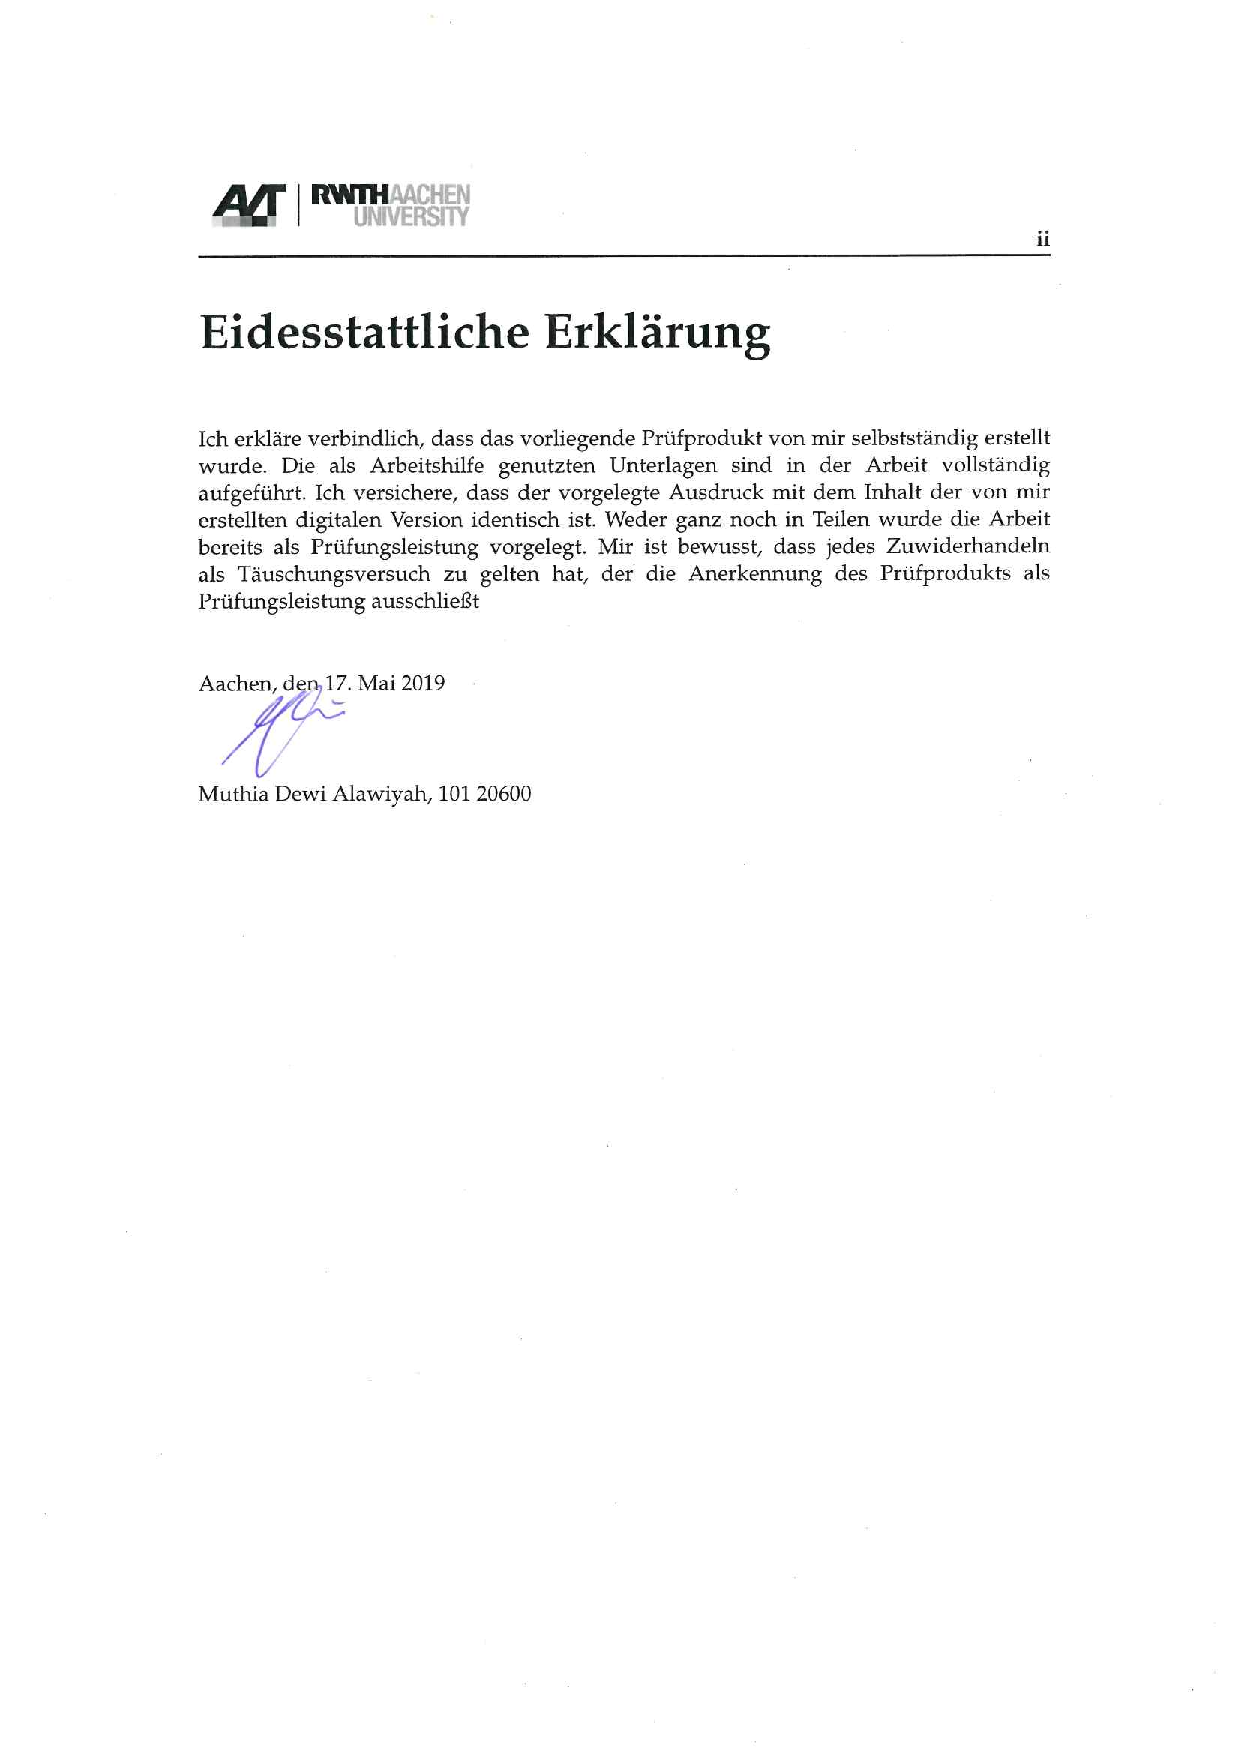
\includepdf[pages=-]{extern/oathstatement.pdf}

%\pdfbookmark{\contentsname}{Inhaltsverzeichnis}
%\setcounter{page}{1}
\makeatletter
\pdfbookmark{\contentsname}{Inhaltsverzeichnis}
\makeatother
\tableofcontents

\clearpage
\begingroup %No page break after \listoffigures
   \let\cleardoublepage\relax  % book
   \let\clearpage\relax        % report
    \phantomsection
    \addcontentsline{toc}{chapter}{\protect\numberline{}Abbildungsverzeichnis}
    \listoffigures
\endgroup

%Die �bersicht sollte in englischer und in deutscher Sprache verfasst werden
%the abstract should include an english and a german version
%%!TEX root = ./main.tex

% This file is part of the i10 thesis template developed and used by the
% Media Computing Group at RWTH Aachen University.
% The current version of this template can be obtained at
% <http://www.media.informatik.rwth-aachen.de/karrer.html>.

\loadgeometry{myAbstract}

\chapter*{Abstract\markboth{Abstract}{Abstract}}
\addcontentsline{toc}{chapter}{\protect\numberline{}Abstract}
\label{abstract}

Die BioLector Technologie wird am Lehrstuhl für Bioverfahrenstechnik seit 2005 eingesetzt. Die Messtechnik erlaubt es, Fluoreszenz und Streulicht in einer Kombination von Emissions- und Exzitationswellenlängen in einer Mikrotiterplatte zu messen \citep{doi:10.1002/bit.20573}. In dem ursprünglichen BioLector Aufbau kommt für die Messung eine Kombination eines Spektrografen und einem Detektor zum Einsatz. Für diesen Aufbau wurde im Jahr 2016 eine externe Software entwickelt, die eine robuste Messung erlaubt. Im gleichen Jahr wurde unabhängig davon eine Modifikation veröffentlicht, die es ermöglicht, zweidimensionale Fluoreszenzspektren aufzunehmen \citep{doi:10.1002/biot.201600515}. Durch den Einbau einer CCD Kamera können so für die Emissionswellenlänge alle Wellenlängen des sichtbaren Lichtes detektiert werden. Je länger die Integrationszeit ist, desto höher ist die aufgenommene Intensität des Streulichtes und der Fluoreszenz. Doch es ist empfehlenswert, keine sehr hohen Intensitäten aufzunehmen, um die CCD Kamera zu schonen. Das heißt, zur Erkennung geringkonzentrierter Fluorophore soll das Streulicht, dass eine deutlich höhere Intensität zeigt, zunächst ausgeblendet werden. Danach kann ebenfalls die Integrationszeit verlängert werden. Dafür wird statt dem feststehenden Brechungsgitter ein bewegliches Gitter im Emissionsmonochromator eingebaut, der das zurückgeworfene Licht auf die Kamera auftrennt und dadurch auswählen kann, welche Wellenlängen aufgenommen werden. Dieser neue Messstand erfordert eine entsprechende neue Software.

Ziel dieser Studienarbeit ist die Analyse zur Umsetzung einer Integration des neuen Messtandes inklusive beweglichem Gitter im Emissionsmonochromator in die vorhandene, extern geschriebene Software. Dafür werden zunächst das Messprinzip des konventionellen sowie des 2D-BioLectors vorgestellt. Anschließend werden zentrale Abläufe der vorhandenen in LabVIEW geschriebenen Software für den konventionellen BioLector und sowie für den zu integrierenden Messstand beschrieben. Dazu gehören die Software-Struktur, die eingesetzten Module und ebenfalls der Ablauf des Messverfahrens. Danach werden die Unterschiede der Anlagen ausgearbeitet und mögliche Schritte zur Integration vorgestellt. Abschließend soll der Aufwand zur Integration der Software abgeschätzt werden. Hierbei soll vor allem auf die Übertragbarkeit der eingesetzten \textit{Producer Consumer} Strukturen, sowie das Verhindern von \textit{Race Conditions} auf den neuen Messstand eingegangen werden. Da dieser zudem eine vielfach höhere Menge an Daten produziert, soll ebenfalls eine geeignete Lösung zur Datenspeicherung vorgestellt werden.

\loadgeometry{myText}


%--------------------------------------------------------------

%In der Arbeit verwendete Konventionen (Formelsatz, Definitionen, etc.)
%conventions applied in the thesis (AE/BE, definitions, etc.)
%%!TEX root = ./main.tex
%
% This file is part of the i10 thesis template developed and used by the
% Media Computing Group at RWTH Aachen University.
% The current version of this template can be obtained at
% <http://www.media.informatik.rwth-aachen.de/karrer.html>.

\chapter*{Conventions\markboth{Conventions}{Conventions}}
\addcontentsline{toc}{chapter}{\protect\numberline{}Conventions}

Throughout this thesis we use the following conventions.



\bigskip

\emph{Text conventions}

Definitions of technical terms or short excursus are set off in coloured boxes.

\myDefBox{Excursus}
{Excursus are detailed discussions of a particular point in a book, usually in an appendix, or digressions in a written text.}
\vspace{5mm} %5mm vertical space

Source code and implementation symbols are written in typewriter-style text.

\texttt{myClass}
\vspace{5mm} %5mm vertical space

The whole thesis is written in Canadian English.
\vspace{5mm} %5mm vertical space

Download links are set off in coloured boxes.

\myDownloadURL{File: myFile}{file_number.file}{file \myUnderscore number.file}

%\pagebreak

%\emph{Formula conventions}





%--------------------------------------------------------------
\mainmatter

%!TEX root = ./main.tex
%
% This file is part of the i10 thesis template developed and used by the
% Media Computing Group at RWTH Aachen University.
% The current version of this template can be obtained at
% <https://hci.rwth-aachen.de/karrer_thesistemplate>.

\chapter{Aufgabenanalyse}

In diesem Abschnitt widergebe ich die Aufgabenstellung in eigenen Worten. Nachher folgt eine genaue Analyse des angeforderten Algorithmus sowie die Restriktionen.

Im Rahmen der Aufgabenstellung ist ein Programm zur vereinfachten Texteingabe mit Hilfe einer numerischen Tastatur zu entwickeln. Eine Software, die dieses Problem löst, ist unter dem Namen T9 bekannt. Die Tastatur verfügt nur über folgende Tasten: 1234567890*\# . Die möglichen Eingaben des Programms "T9" sind 12 unterschiedliche Buchstaben in der Menge $E:=\{1,2,...,9,0,*,\# ,Enter\}$. Die Enter-Taste wird in allen Konsolenprogrammen benötigt, um Eingaben zu bestätigen.

Mit der Menge E sollen Wörter bzw. Sätze in Großbuchstaben geschrieben und mit Hilfe eines Wörterbuchs erkannt werden.
Die Zuordnung der Buchstabe nzu den numerischen Taste ist wie folgt festgelegt:
\newline
\begin{table}[h!]
\begin{tabular}{ccc}
$\sqcup$ & ABC & DEF  \\
1        & 2   & 3    \\
GHI      & JKL & MNO  \\
4        & 5   & 6    \\
PQRS     & TUV & WXYZ \\
7        & 8   & 9    \\
\textit{Ja}       & .   & \textit{NEIN} \\
*        & 0   & \#  
\end{tabular}
\end{table}
\newline
Das Programm kann dynamisch erweitert werden, indem man Wörter zum Wörterbuch hinzufügt.

\section{Algorithmus}
\label{algorithmus}

Bei der Eingabe wird zwischen zwei Modies unterschieden: Einfachmodus und Explizitmodus. Die beiden Modus unterscheiden sich in der Interpretation der Eingabemenge E.
Das Programm bildet beliebig viele Sätze mit Einschränkung der möglichen Eingaben (s. Restriktionen).
Alle Einträge im Wörterbuch, die nur per Explizitmodus gespeichert worden sind, werden Extern in einer Textdatei gespeichert und bei jedem erneuten Ausführen des Programms wieder Aufgerufen und für Textsuche verwendet.

\subsection{Modus der normalen Texteingabe}
\label{normal}

Für die Texteingabe wird pro Buchstabe nur eine Zifferntaste gedrückt.

Beispieleingabe:
\begin{table}[h!]
\begin{tabular}{lllllllll}
S & O & F & T & W & A & R & E & $\sqcup$ \\
7 & 6 & 3 & 8 & 9 & 2 & 7 & 1 & 1
\end{tabular}
\end{table}
\newline
Beim Eingeben der Leertaste 1 oder der Punkt 0 wird Ende des Wortes bzw. des Satzes signalisiert.
Das Wort wird anhand der Ziffernfolge im Wörterbuch gesucht.
Falls mehrere Wörter die gleiche Ziffernfolge haben, wird das Häufigste Wort vorgeschlagen.
Falls kein Eintrag im Wörterbuch gefunden wurde, wird der Nuzter zum Explizitmodus weitergeleitet.

\subsection{Explizitmodus}
\label{explizit}

Im Explizitmodus wird keine Suche im Wörterbuch stattfinden. Der Nuzter wird stattdessen aufgefordert, Wörter zum Speichern im Wörterbuch einzugeben.
Die Eingabe wird explizit erfolgen. D.h. die genauen Buchstaben werden eingegeben.

Beispieleingabe:
\newline
\begin{table}[h!]
\begin{tabular}{lllll}
W  & O  & R  & T  & $\sqcup$ \\
91 & 63 & 73 & 81 & 1       
\end{tabular}
\end{table}

Hier signalisieren auch Leertaste 1 oder Punkt 0 Ende des Wortes bzw. des Satzes.
Für jede Buchstabe werden zwei Ziffern benötigt. Eine für Ort im Ziffernblock und die Zweite für den Ort innerhalb der gewählten Ziffernblock.

\subsection{Wörter und Sätze}
Das Programm unterscheidet zwischen Wörter und Sätze. Falls die Eingabe mit einem Punkt(0) endet wird Ende des Satzes signalisiert und im Anschluss das ganze Satz gezeigt.
Falls die Eingabe mit einer Leertaste(1) endet wird Ende des Wortes signalisiert und im Anschluss weiergeschrieben bis Ende des Satzes eingegben wird.


\subsection{das Wörterbuch}
\label{dic}
Alle Einträge des Wörterbuchs werden in einer HashMap sowie einer Baumstruktur gespeichert. Der Schlüssel der jeweiligen Einträge ist der explizite Zifferncode aus der Menge \{2, 3, 4, 5, 6, 7, 8, 9\} Wobei Leertast (0) oder Punkt(0) nicht gespeichert werden.
Somit sind die Einträge im Wörterbuch eineindeutig abgebildet und somit einfach zu finden.
Am Anfang bzw. am Ende des Programmablaufs wird das Wörterbuch in eine Textdatei gespeichert bzw. gelesen.
Beim speichern werden alle Einträge des Wörterbuchs Zeilenweise in der Textdatei geschrieben.
Eine Zeile hat folgendes Muster: \textless Code\textgreater \textless Wort\textgreater \textless Häufigkeit\textgreater 
\newline
Beispile: 91637333 WORF 2

\subsection{Benutzerdialog im Hauptprogramm}
Die Benutzereingabe bzw. Ausgabe erfolgt mit einer Konsole. Die Taste Enter beendet die Eingabe.

\textbf{Falls ein Satz nur mit einem Punkt eingegeben wurde, wird das Programm beendet.}

\section{Restriktionen}

\subsection{Restriktionen der Eingabedatei}
Eine Textdatei enthält Zeilenweise gespeicherte Einträge vom Wörterbuch.
Solche Textdatei muss folgende Restriktionen erfüllen:
\begin{itemize}
    \item Die Eingabedatei muss existieren und lesbar sein, sonst wird kein Wörterbuch geladen.
    \item Die Eingabedatei soll in Form einer Textdatei mit lebarer ASCII-Text sein.
    \item Pro Eintrag des Wörterbuchs wird eine Zeile in der Textdatei gespeichert und durch Zeilenvorschub getrennt.
    \item Das Muster Pro Eintrag muss wie im Abschnitt 1.1.4 (\nameref{dic}) beschrieben übereinstimmen
    \item Die Eingabedatei darf keine doppelte Einträge enthalten
    \item Die Textdatei muss mit einem normalen Texteditor bearbeitbar sein.
    \item Die Ziffernfolge für jeden Eintrag muss mit der Menge der möglichen Eingaben im Benutzerdialog enthalten sein.
\end{itemize}

Falls die Eingabedatei nicht konform mit der oben genannten Punkten, wird die Datei nicht geladen.
Andernfalls wird die im Programm angegebene Textdatei geladen.

\subsection{Restriktionen der Benutzereingabe}
Wie oben in den Abschnitten \textbf{\nameref{normal}} und \textbf{\nameref{explizit}} angegeben haben die Konsoleneingaben folgende Restriktionen:
\begin{itemize}
    \item Alle Eingaben sind nur aus der Menge $E:=\{1,2,...,9,0,*,\# ,Enter\}$
    \item Eine Explizite Ziffernfolge muss konform mit der vorgeschriebenen Zuordnung der Tastatur in der Aufgabenanalyse
    \item Kein Wort sollte aus nur einer Leertaste (1) oder nur einem Punkt (0) bestehen
\end{itemize}  	%% Analyse

%!TEX root = ./main.tex
%
% This file is part of the i10 thesis template developed and used by the
% Media Computing Group at RWTH Aachen University.
% The current version of this template can be obtained at
% <https://hci.rwth-aachen.de/karrer_thesistemplate>.

\chapter{Verfahrensbeschreibung}

In diesem Abschnitt folgt eine genaure Untersuchung der im Programm enthaltenen Funktionalitäten. 

Das Programm hat zwei elementare Funktionalitäten. Die Suche nach Wortvorschläge im Wörterbuch anhand einer einfachen Ziffernfolge sowie die Filterung und die Interpretation von Eingaben von Expliziten Ziffernfolgen.
\section{Die Suche im normalen Modus der Texteingabe}
\label{Suche}

Für eine effiziente Suche im Wörterbuch wird eine Datenstruktur eines Baumes verwendet. Für jede Ziffer in der expliziten Ziffernfolge eines Wortes wird einen Knotenpunkt im Baum erstellt. Dies vereinfacht die Suche erheblich im Vergleich mit der Datenstruktur einer Tabelle. 
Ein Beispielbaum mit folgenden gespeicherten Wörtern
\{ZNRF, WORF, ZO, Z, Y, A\}

\begin{tikzpicture}[->,>=stealth',level/.style={sibling distance = 5cm/#1,
  level distance = 1.5cm}] 
\node [arn_x] {}
    child{ node [arn_n] {9}
        child{ node [arn_r] {1} 
                child{ node [arn_n] {6} 
                	child{ node [arn_r] {3}
                	    child{ node [arn_n] {7}
                	        child{ node [arn_r] {3}
                	            child{ node [arn_n] {3}
                	                child{ node [arn_r] {3}
                	                }
                	            }
                	        }
                	    }
                	}
                }                            
        }
        child{ node [arn_r] {3}}
    	child{ node [arn_r] {4} 
                child{ node [arn_n] {6} 
                	child{ node [arn_r] {2}
                	    child{ node [arn_n] {3}}
                	    child{ node [arn_n] {7}
                	        child{ node [arn_r] {3}
                	            child{ node [arn_n] {3}
                	                child{ node [arn_r] {3}
                	                }
                	            }
                	        }
                	    }
                	}
                }                            
        }
    }
    child{ node [arn_n] {2}
        child{ node [arn_r] {1}}
    }
; 
\end{tikzpicture}

Die Knotenpunkte im Baum Bilden die Menge der expliziten Ziffernfolgen eineindeutig ab. Alle Knoten mit der Endziffer eines Wortes enthält die Häufigkeit des Wortes als integer Zahl gespeichert.
Schwarze und rote Knoten im Baum sind identisch.
Bei der Suche im Baum werden alle schwarzen Knoten besucht, die einen identischen Index mit der vorligenden Ziffer haben. Die roten Knoten werden für die Identifikation des Wortes benötigt. Deswegen werden die roten Knoten direkt unterhalb eines besuchten schwarzen Knoten immer besucht. Die roten Knoten sind die Endziffer eines Wortes. Aus diesem Grund sind die Häufigkeiten (n) in diesem Knoten als Integerzahl gespeichert. Alle anderen Knoten haben die Häufigkeit (n=0).

Die Suche im Baum erfolgt nach dem Prinzip von Sammelkorb. Alle Endknoten der gefundenen Wörter werden gesammelt und anschließend ihre Häufigkeiten verglichen. Der Knotenpunkt mit max(n) wird zurückgegben.
Um aus diesem Knoten ein Wort zu bilden, durchläuft das Programm die Knoten rückwärts bis zum Wurzel und speichert dabei die Indexen der Knoten. Die sich ergebende Ziffernfolge wird umgekehrt und in einem Wort umgewandelt.
Falls alle gefunden Knoten die Häufigkeit (n=0) haben, ist kein Wort gefunden, die die Ziffernfolge entspricht.

\section{Wortbildung und Interpretation}
Das Wörterbuch ist in der Lage, Wörter als explizite Ziffernfolgen als Buchstaben in Großschreibung zu interpretieren.
Für diese Umwandlung von Ziffern zu Buchstaben sind if-else-Abzweigung nötig. Diese Unterscheiden dann die Ziffernfolgen voneinander.
Um festzustellen, dass die Eingaben der Nutzer auf der Konsole stimmig mit der Anforderungen sind, werden sie in der Konsole zuerst von Punkten oder Leertasten am Ende gefiltert und nach Richtigkeit gecheckt. 	%% Verfahrensbeschreibung

%!TEX root = ./main.tex
%
% This file is part of the i10 thesis template developed and used by the
% Media Computing Group at RWTH Aachen University.
% The current version of this template can be obtained at
% <https://hci.rwth-aachen.de/karrer_thesistemplate>.

\chapter{Programmkonzeption}

In diesem Abschnitt gehe ich auf die Konzeptionelle Phase des Programms näher. Dabei beschreibe ich die Programmstruktur mittels UML-Klassendiagramme. Mit einer Sequenzdiagramm ist das Programmablauf gut veranschaulicht worden. Schließlich folgt eine genauere Beschreibung der verwendeten Methoden mittels Nassi-Schneiderman-Diagrammen.

\section{Klassen}
Das Programm beinhaltet folgende Klassen:

\subsection{\texttt{Main}}
    
    Die Hauptklasse für das Programm T9.
    Diese Klasse beinhaltet die Einsprungfunktion des gesamten Programms. Es Wird ein Wörterbuch sowie eine Konsole erstellt. die Konsole wird gestartet und nach Ende der Nutzerinteraktion wieder beendet.
    
\subsection{\texttt{Konsole}}
    
    Diese Klasse ist die Konsole für die Nutzerinteraktion. Beim Starten der Konsole wird das Wörterbuch aus einer Datei geladen. Bei diesem Vorgang wird der Nutzer benachrichtigt, ob das Wörterbuch geladen ist oder nicht.
    Die Konsole verwaltet die Eingaben und Ausgaben des Programms. Die Eingaben vom Nutzer werden gefiltert und nach Richtigkeit geprüft. Im Falle einer Falschen Eingabe, wird ein Fehler auf der Konsole mit folgender Form gezeigt:\newline
    Falsche Eingabe\newline
    \textless Grund\textgreater
    \newline
    Mögliche Ausgaben:
    \begin{enumerate}
        \item Kein Woerterbuch geladen
        \item Woerterbuch geladn
        \item Kein passendes Wort gespeichert. Eingabe im Explizitmodus:
        \item \textless Wort-Vorschlag\textgreater
        \item Wort ok?
        \item Wort gespeichert
        \item Der Satz lautet \textless gebildeter Satz\textgreater
        \item Programmende.
    \end{enumerate}{}
    Alle Ausgaben mit den \textless \textgreater -Klammern sind dynamisch.
    
    
    
\subsection{\texttt{Woerterbuch}}
    
    Diese Klasse repräsentiert das Wörterbuch des Programms T9. Die Klasse beinhaltet eine Tabelle in Form einer HashMap, um die Speicherung des Wörterbuchs sowie das Lesen aus einer Textdatei zu vereinfachen.
    Die Klasse beinhaltet einen \textit{Baum} für die Textsuche, eine integer Zahl als festgelegte Größe des Wörterbuches und eine Pfadangabe als String für die Textdatei des Wörterbuchs.
    Die Methode \texttt{ladeBib} lädt das Wörterbuch aus der Textdatei. Dabei wird bei Fehler keine Datei geladen.
    Die Methode \texttt{speichereBib} speichert das Woerterbuch in der Textdatei. Bei Fehler wird nicht gespeichert und keine Fehlermeldung zurückgegeben.
    Für die Suche sowie Hinzufügen eines Wortes wird in der Klasse \texttt{Baum} die Suchfunktion sowie die \texttt{add}-Funktion aufgerufen. \texttt{add} fügt ein Wort sowohl im HashMap als auch im Baum.
    Beim Erstellen eines Baumes wird die Methode \texttt{makeTree} aufgerufen, die ein Baum für die vereinfachte Suche erstellt. Dabei werden alle Einträge im HashMap gelesen und im Baum gespeichert.
    Die Verwandlung von einer expliziten Ziffernfolge in einem Wort im Alphabet übernimmt die statische Methode \texttt{makeWord}. Diese Methode wird auch in der Klasse \texttt{Baum} verwendet, um gesuchte Ziffernfolgen umzuwandeln.
    
\subsection{\texttt{Baum}}
    
    Beinhaltet alle Einträge des Wörterbuchs im Form von Baumstruktur. Alle Knoten sind von der Klasse \texttt{Node}.
    Der Wurzelknoten ist eine ArrayList \textbf{root}, die alle Knoten enthält. \texttt{search} bekommt ein \textbf{key}, ein String von Ziffernfolge, und sucht rekursiv nach einem Treffer im Baum. Falls kein Treffer gefunden ist wird der String -1 zurückgegben. Um Wörter aus einem Endknoten zu konstruieren, wird \texttt{constructWord} mit einem Knoten aufgerufen. Diese Methode sucht alle Elternknoten der Reihe nach und speichert die Indexen der Knoten in einem String. Der String wird rückwärts umgewandelt und zu einem Wort mit Hilfe von \texttt{makeWord} interpretiert. Um ein Wort im Baum hinzufügen wird \texttt{add} aufgerufen. Diese Methode Wird rekursiv aufgerufen um Knoten im Baum hinzufügen oder falls schon vorhanden aktualisieren. Die Methode bekommt also eine explizite Ziffernfolge und ein Häufigkeit des Wortes. Falls keine Häufigkeit von einem Wort existiert wird die Methode 0 bekommen. Falls die Häufigkeit 0 ist, wird jedesmal, wenn ein bereits im Baum gespeichertes Wort erneut ausgewählt wird, wird seine Häufigkeit um eins erhöht.
    
\subsection{\texttt{Node}}
    
    Die Klasse repräsentiert einen Knoten im \texttt{Baum}. Sie beinhaltet Integerzahl n als Häufigkeit sowie ein Integerzahl als Index, ArrayList aus Node für allen Kindknoten und ein Node für einen Elternknoten.
    Die Methode \texttt{has} prüft nach Existenz eines Kindknotens und die Methode \texttt{get} liefert einer der Kindknoten mit einem eingegebenen Index.


\clearpage

\section{UML-Klassendiagramm}
%
%\begin{figure}[!ht]
%\centering
%\includegraphics[width=\textwidth]{../../src/resources/uml.png}
%\caption[UML-Klassendiagramm]{UML-Klassendiagramm der implementierten Klassen}
%\end{figure}

\section{Aktivitätsdiagramm zum Programmablauf}
Eine detaillierte Beschreibung des Programmablaufs anhand eines Aktivitätsdiagramm. Dies verdeutlich den Lebenszyklus mit den Kontroll-Beziehungen.
\begin{figure}[H]
\centering
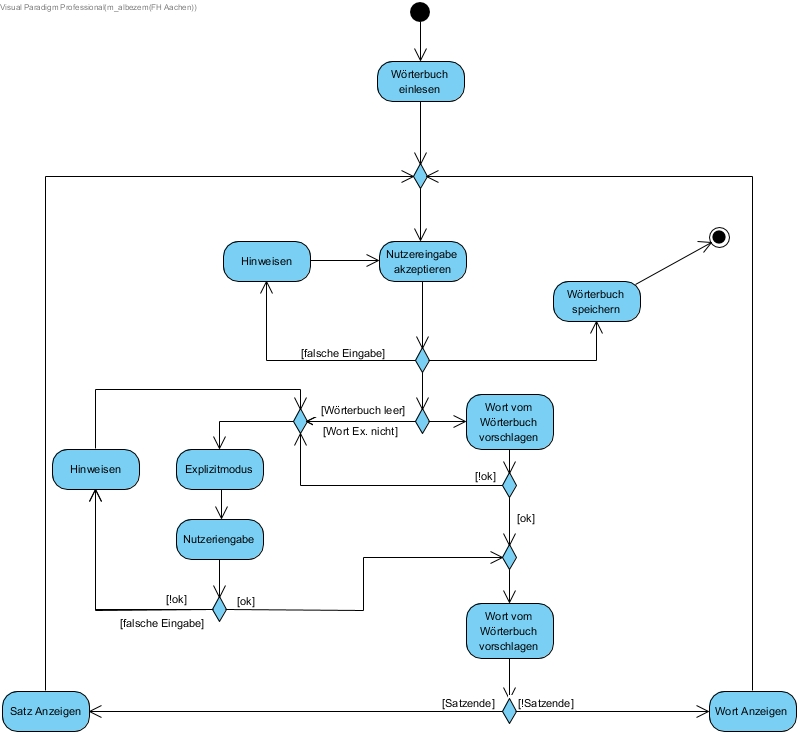
\includegraphics[width=1.\columnwidth]{images/activitydiagramm.jpg}
\caption[UML-Sequenzdiagramm]{UML-Aktivitätsdiagramm zum Programmablauf}
\end{figure}

\section{Beschreibung der Methoden}
Eine detailierte Beschreibung der Methoden folgt in Form von Nassi-Schneiderman-Diagrammen bzw. Struktogrammen.

\begin{figure}[!ht]
\centering
\includegraphics[width=\textwidth]{../../src/resources/toUpper.png}
\caption[UML-Klassendiagramm]{Algorithmus zur Umwandlung von Buchstaben in einem String zu Großbuchstaben}
\end{figure}

\begin{figure}[!ht]
\centering
\includegraphics[width=\textwidth]{../../src/resources/readInputFile.png}
\caption[UML-Klassendiagramm]{Algorithmus zum Lesen von Input-Datei}
\end{figure}
	%% Konzept

%!TEX root = ./main.tex
%
% This file is part of the i10 thesis template developed and used by the
% Media Computing Group at RWTH Aachen University.
% The current version of this template can be obtained at
% <https://hci.rwth-aachen.de/karrer_thesistemplate>.

\chapter{Entwicklungsumgebung}
\label{chap:Env}

Die Entwicklung und Tests der Software wurden auf einem System mit folgender Spezifikation durchgeführt:
\begin{itemize}
\item Betriebsystem: Microsoft Windows 10 Enterprise (64 Bit)
\item  Prozessor: AMD FX(tm)-8350 Eight-Core Processor, 4000 MHz, 4 Kern(e), 8 logische(r) Prozessor(en)
\item Installierter physischer Speicher (RAM) 16,0 GB
\item Grafikkarte: NVIDIA GeForce 210
\end{itemize}

Weitere Spezifikationen:
\begin{itemize}
\item Die Software wurde mit der Programmiersprache Java in der Version 11.0.2 entwickelt. Verwendet wurde die IDE Intellij IDEA Community 2019.3.2.
\item Zur Erstellung von Textdateien wurde der Texteditor Notepad++ benutzt.
\item Für die Klassen- und Sequenzdiagramm wurde das Programm Visual Pardigm 16 verwendet.
\item Zur Erstellung von Nassi-Schneiderman-Diagrammen wurde Java-Editor18.23 verwendet.
\item Zur Erstellung dieser Dokumentation wurde MiKTeX 2.9 bzw. ein Online-Latex-Editor Overleaf verwendet.
\end{itemize}	%% Entwicklungsumgebung

%!TEX root = ./main.tex
%
% This file is part of the i10 thesis template developed and used by the
% Media Computing Group at RWTH Aachen University.
% The current version of this template can be obtained at
% <https://hci.rwth-aachen.de/karrer_thesistemplate>.

\chapter{Benutzeranleitung}

\section{Verzeichnisstuktur}

\begin{itemize}
    \item README.md ist die Readme-Datei für das Projekt
    \item \texttt{src} : In diesem Verzeichnis befinden sich alle Testklassen, sowie der Quellcode des Programms
    \item \texttt{out}: In diesem Verzeichnis befinden sich alle kompilierten Java Dateien
    \item \texttt{doc} : In diesem Verzeichnis befindet sich die Programm-Dokumentation
    \begin{itemize}
        \item \texttt{javadoc}: In diesem Verzeichnis liegt die generierte Entwicklerdokumentation
        \item \texttt{documentation}: In diesem Verzeichnis liegen die Latex-Dateien zur Erzeugung dieser Dokumentation
        \item \texttt{Dokumentation.pdf}: Dieses Dokument
    \end{itemize}
    \item \texttt{tests}: In diesem Verzeichnis befinden sich Beispiele für die Eingabe-, Ausgabe und Fehlerdateien
    \begin{itemize}
        \item \texttt{ihk} für Beispiele aus der Aufgabenstellung
        \item \texttt{itests} für selbst ausgesuchte Beispiele 
    \end{itemize}
\end{itemize}

\section{Systemanforderungen}

Die Software ist unter Java JRE 11 (Java Runtime Environment Version 11) ausführbar. Dafür muss die genannte Java-Version oder höher auf der Maschine installiert sein. Außerdem sollte beachtet werden, dass Java nicht abwährtskompatibel ist und entsprechend keine ältere Version verwendet werden sollte.\\
Das Programm wurde wie im Kapitel \ref{chap:Env} beschrieben entwickelt.\\
Die Ausführbarkeit wird unter dem genannten Voraussetzungen garantiert.\\
Zudem kann das Programm unter Linux/Unix mit oben gennanten Vorausetzungen (Java-Version) ausgeführt werden.



\section{Benutzung der Kommandozeile unter Windows}


Mit Hilfe der Kommandozeile (Eingabeaufforderung unter Windows bzw. Shell unter Linux/Unix) müssen Sie in das Verzeichnis \texttt{\texttildelow \textbackslash out\textbackslash artifacts\textbackslash makeUpper\textunderscore jar\textbackslash}. 
Das Programm wird wie folgt gestartet: 

Beispielaufruf: \texttt{java -jar T9.jar} falls das Programm in Kommandozeile-Modus aufgerufen werden sollte

Beispielaufruf: \texttt{java -jar T9.jar -i testfall.txt} falls das Programm mit einer Eingabedatei testfall.txt ausgeführt werden sollte.


\section{Die Ausführung der Testfälle}
Je nach Betriebssystem liegt ein Bash- oder Shell-Script zur Verfügung, um die Testfälle im Verzeichnis \textit{tests} automatisiert auszuführen.


Die Dateien (run\textunderscore tests.bat bzw. run\textunderscore test.sh) führen die oben genannten Befehle automatisiert mit allen Testfällen im Verzeichnis \texttt{tests} aus. Dabei muss die Pfadeingabe zur .jar-Datei und der zur Testdatei(en) korrekt sein. 
Für nähere Informationen zu Testfällen siehe Kapitel  \ref{chap:Testing}
	%% Benutzeranleitung

%!TEX root = ./main.tex
%
% This file is part of the i10 thesis template developed and used by the
% Media Computing Group at RWTH Aachen University.
% The current version of this template can be obtained at
% <https://hci.rwth-aachen.de/karrer_thesistemplate>.

\chapter{Testfälle und Diskussion}
\label{chap:Testing}
\section{Konvention}
Die Testfälle sind unterteilt in IHK-Beispliele und selbst erstellte Tests. Die Testdateien haben folgende Benennung: Die Bezeichnung [0-9] steht für eine Zahl aus dem Bereich von 0 bis 9
\begin{itemize}
\item  E[0-9][0-9][0-9].txt für\textbf{ Eingabedateien}
\item  E[0-9][0-9][0-9].output.txt für\textbf{ Ausgabedateien}
\item  E[0-9][0-9][0-9].error.txt für\textbf{ Fehlerdateien}
\end{itemize}
Es wird grundsätzlich immer zu jeder Eingabedatei eine Ausgabe- und Fehlerdatei erzeugt.
Hat das Programm keine Fehler bzw. keine Ausgabe erzeugt, sind die Dateien \textbf{leer}.
Beispielsweise erzeugt die Eingabedate E001.txt nach meiner Konvention die Ausgabedatei E001.output.txt und die Fehlerdatei E001.error.txt.


\section{IHK-Beispiele}
Nachfolgend sind die Beispieler von der IHK-Aufgabenstellung mit aufgelistet. Aus den Kommentaren in der Eingabedateien ist eine genauere Beschreibung zu sehen.
%Im ersten Beispiel wurde das Programm mit einem leeren Wörterbuch geöffnet und die Wörter FES, DER, EIN, IST, HUT im Wörterbuch gespeichert. Mit diesem ersten Beispiel wird die Konsoleeingabe, die Unterscheidung zwischen Sätze und Wörter, die Suche im Wörterbuch, die Beendung des Programms sowie die Speicherung in einer Textdatei getestet.
%Im zweiten Beispiel wird das Wörterbuch aus der vorigen Beispiel geladen und anschließend erweitert. 
%Im dritten Beispiel wird getestet, ob zwei Wörter mit der gleichen einfachen Zifferncode richtig im Wörterbuch gesucht werden.\\\\


%\verbfilenobox[\mbox{\scriptsize\theVerbboxLineNo:} ]{../../tests/E001.txt}
\begin{itemize}
\item \textbf{Testfall1}: Kein Randwert und kein Sonderfall.
Eingabe: \VerbatimInput[frame=single, numbers=left]{../../tests/E001.txt}
Ausgabe: \VerbatimInput[frame=single, numbers=left]{../../tests/E001.output.txt}
Fehler: Leer

\item \textbf{Testfall2}: einzelne Großbuchstabe
Eingabe: \VerbatimInput[frame=single, numbers=left]{../../tests/E002.txt}
Ausgabe: \VerbatimInput[frame=single, numbers=left]{../../tests/E002.output.txt}
Fehler: Leer

\item \textbf{Testfall 11}: einzelne Sonderzeichen
Eingabe: \VerbatimInput[frame=single, numbers=left]{../../tests/E011.txt}
Ausgabe: \VerbatimInput[frame=single, numbers=left]{../../tests/E011.output.txt}
Fehler:\VerbatimInput[frame=single, numbers=left]{../../tests/E011.error.txt}

\end{itemize}

\cite{UML}
\cite{SWT}

%
%\lstinputlisting[language={}, caption=Ausgabe zu E001]{../../tests/E001.output.txt}
%\lstinputlisting[language={}, caption=Error log zu E001]{../../tests/E001.error.txt}
%
%\lstinputlisting[language={}, caption=Eingabe]{../../tests/E002.txt}
%\lstinputlisting[language={}, caption=Ausgabe]{../../tests/E002.output.txt}
%\lstinputlisting[language={}, caption=Error log]{../../tests/E002.error.txt}
%
%\lstinputlisting[language={}, caption=Eingabe]{../../tests/E003.txt}
%\lstinputlisting[language={}, caption=Ausgabe]{../../tests/E003.output.txt}
%\lstinputlisting[language={}, caption=Error log]{../../tests/E003.error.txt}
%
%\lstinputlisting[language={}, caption=Eingabe]{../../tests/E004.txt}
%\lstinputlisting[language={}, caption=Ausgabe]{../../tests/E004.output.txt}
%\lstinputlisting[language={}, caption=Error log]{../../tests/E004.error.txt}
%
%\lstinputlisting[language={}, caption=Eingabe]{../../tests/E005.txt}
%\lstinputlisting[language={}, caption=Ausgabe]{../../tests/E005.output.txt}
%\lstinputlisting[language={}, caption=Error log]{../../tests/E005.error.txt}
%
%\lstinputlisting[language={}, caption=Eingabe]{../../tests/E006.txt}
%\lstinputlisting[language={}, caption=Ausgabe]{../../tests/E006.output.txt}
%\lstinputlisting[language={}, caption=Error log]{../../tests/E006.error.txt}
%
%\lstinputlisting[language={}, caption=Eingabe]{../../tests/E007.txt}
%\lstinputlisting[language={}, caption=Ausgabe]{../../tests/E007.output.txt}
%\lstinputlisting[language={}, caption=Error log]{../../tests/E007.error.txt}
%
%\lstinputlisting[language={}, caption=Eingabe]{../../tests/E008.txt}
%\lstinputlisting[language={}, caption=Ausgabe]{../../tests/E008.output.txt}
%\lstinputlisting[language={}, caption=Error log]{../../tests/E008.error.txt}
%
%\lstinputlisting[language={}, caption=Eingabe]{../../tests/E009.txt}
%\lstinputlisting[language={}, caption=Ausgabe]{../../tests/E009.output.txt}
%\lstinputlisting[language={}, caption=Error log]{../../tests/E009.error.txt}
%
%\lstinputlisting[language={}, caption=Eingabe]{../../tests/E010.txt}
%\lstinputlisting[language={}, caption=Ausgabe]{../../tests/E010.output.txt}
%\lstinputlisting[language={}, caption=Error log]{../../tests/E010.error.txt}
%
%\lstinputlisting[language={}, caption=Eingabe]{../../tests/E011.txt}
%\lstinputlisting[language={}, caption=Ausgabe]{../../tests/E011.output.txt}
%\lstinputlisting[language={}, caption=Error log]{../../tests/E011.error.txt}

\clearpage

\section{Eigene Beispiele}

\subsection{Äquivalenzklassen}
Nachfolgend sind Testbeispiele aufgelistet, die das Programm weitestgehend funktional testen. Dabei werden die Äquivalenzklassen behandelt, die ich mir in der Konzeptionsphase ausgedacht habe. In Tabelle \ref{tab:tests} sind die Äquivalenzklassen in zulässige und unzulässige Mengen unterteilt. Liegt ein Representant in der unzulässigen Menge, sollte das Programm einen entsprechenden Fehler ausgeben. 

\begin{table}[H]
\begin{tabular}{|l|l|l|l|}
\hline
Name & Zulässige  Bereich & Unzulässige Bereich & Repräsentant \\ \hline
   Buchstaben  &  \{A-Z,a-z,0-9\}                  &     Sonderzeichen                &  Ä            \\ \hline
    Sätze &                    &                    &              \\ \hline
\end{tabular}
\caption{Tabelle mit den Äquivalenzklassen}
\label{tab:tests}
\end{table}


\subsection{Beispiele}
\begin{itemize}
\item \textbf{Testfall1}: Kein Randwert und kein Sonderfall.
Eingabe: \VerbatimInput[frame=single, numbers=left]{../../tests/E001.txt}
Ausgabe: \VerbatimInput[frame=single, numbers=left]{../../tests/E001.output.txt}
Fehler: Leer

\item \textbf{Testfall2}: einzelne Großbuchstabe
Eingabe: \VerbatimInput[frame=single, numbers=left]{../../tests/E002.txt}
Ausgabe: \VerbatimInput[frame=single, numbers=left]{../../tests/E002.output.txt}
Fehler: Leer

\item \textbf{Testfall 11}: einzelne Sonderzeichen
Eingabe: \VerbatimInput[frame=single, numbers=left]{../../tests/E011.txt}
Ausgabe: \VerbatimInput[frame=single, numbers=left]{../../tests/E011.output.txt}
Fehler:\VerbatimInput[frame=single, numbers=left]{../../tests/E011.error.txt}

\end{itemize}


%Ich habe folgende Beispiele als JUnit-Testklassen ausgedacht:
%\begin{enumerate}
%    \item Ein Wörterbuch laden, das nicht im Verzeichnis existiert
%    \item Ein Wörterbuch laden, das mehr als ein Eintrag in einer Zeile enthält. Hier wird der Zeilenvorschub getestet
%    \item Ein Wörterbuch mit zu langer Codewort
%    \item Ein Wörterbuch mit Wort in Kleinschreibung oder aus Buchstaben
%    \item Ein Wörterbuch mit Übereinstimmung von Code und Wort
%    \item Ein Wörterbuch mit doppelten Einträgen
%    \item Ein Wörterbuch, das zwar leer ist aber Zeilenvorschub enthält
%    \item Ein Wörterbuch, das die korrekten Einbaben hat.
%    \item Ein zu großes Wörterbuch
%    \item Das Programm hat keine Textdatei zum Speichern sondern andere Extension
%    \item Das Programm bekommt einen neuen Namen einer Textdatei zum Speichern
%    \item \texttt{testbib1.text} enthält ein Beispiel aus dem Baum im Abschnitt 2. Der nach dem Laden entstandene Baum wird weist eine Struktur, die eindeutig Ziffernwörter abblidet. Dies wird mit den zwie Wörtern \textbf{ZNRF} und \textbf{WORF} getestet. Außerdem hat ZNRF die Häufigkeit 2 und WORF die Häufigkeit 1. Somit sollte ZRNF gewählt werden. In \texttt{textbib2.text} sollte WORF gewählt werden, da sie Häufigkeit 2 hat und ZRNF Häufigkeit 1 hat.
%    In diesem Baum wird auch getestet, ob die Nachbarknoten verglichen werden. Für die suche nach \textbf{ZO} sollte nicht \textbf{ZN} rauskommen.
%\end{enumerate}
%
%\lstinputlisting[language={}, caption=Testbeispiel 2 - Wörterbuch]{testfaelle/falsebib1.text}
%\lstinputlisting[language={}, caption=Testbeispiel 3 - Wörterbuch]{testfaelle/falsebib3.text}
%\lstinputlisting[language={}, caption=Testbeispiel 4 - Wörterbuch]{testfaelle/falsebib4.text}
%\lstinputlisting[language={}, caption=Testbeispiel 5 - Wörterbuch]{testfaelle/falsebib5.text}
%\lstinputlisting[language={}, caption=Testbeispiel 6 - Wörterbuch]{testfaelle/falsebib6.text}
%\lstinputlisting[language={}, caption=Testbeispiel 8 - Wörterbuch]{testfaelle/truebib.text}
%\lstinputlisting[language={}, caption=Testbaum 1 - Baum]{testfaelle/testbib1.text}
%\lstinputlisting[language={}, caption=Testbaum 2 - Baum]{testfaelle/testbib2.text}
%\lstinputlisting[language=java, caption=Klasse \texttt{WoerterbuchTest}]{sourcecode/WoerterbuchTest.java} 	%% Testdiskussion

%!TEX root = ./main.tex
%
% This file is part of the i10 thesis template developed and used by the
% Media Computing Group at RWTH Aachen University.
% The current version of this template can be obtained at
% <https://hci.rwth-aachen.de/karrer_thesistemplate>.

\chapter{Abweichungen des Prüfungsproduktes vom Konzept}

Bei der Umsetzung des Konzeptes in das Programmsystem wurden einige kleine Änderungen vorgenommen. Folgende Änderungen am Konzept sind anzuführen:

\begin{itemize}
    \item Die Baumstruktur in der Klasse \texttt{Baum} speichert die Wörter mit ihrem expliziten Ziffernfolge. Dies liegt daran, dass die Reihenfolge der Buchstaben in einem Knoten nicht ausreicht, um Wörter eineindeutig zuzuordnen.
    \item Die Klassenstruktur hat noch zusätzliche Hilfsfunktionen wie \texttt{nutzerinteraktion()} in \textbf{Konsole} oder \texttt{makeWord()} in \textbf{Woerterbuch}
    \item Die Nassi-Schneidermann-Diagrammen ersetzen den im Prüfungsproduktes aufgeführten Pseudocode.
\end{itemize}	%% Abweichung von Konzeptionsphase

%!TEX root = ./main.tex
%
% This file is part of the i10 thesis template developed and used by the
% Media Computing Group at RWTH Aachen University.
% The current version of this template can be obtained at
% <https://hci.rwth-aachen.de/karrer_thesistemplate>.

\chapter{Zusammenfassung und Ausblick}

Es kann zahlreiche Erweiterungen zu dieser Software geben. Möglichkeiten wären beispielsweise, eine erweiterte Interpretation der Tasten, um Zahlen darzustellen, Darstellung von Klein und Großschreibung.

Für die Eingabe sowie die Ausgabe könnte eine graphische Oberfläche implementiert werden. Dadurch könnte der Anwender die Ausgabe graphisch besser sehen.

Das Programm speichert die Eingaben von Nutzer im Wörterbuch nur bei einer expliziten Eingabe von Zifferncode. Dies kann einfacher gestaltet werden, indem die Wortvorschläge nicht nur aus dem Wörterbuch vorgeschlagen werden, sondern aus dem Tippverhalten des Nutzers. Ein Wörterbuch bestehend aus Konstellationen von den Häufigsten benutzen Buchstaben können vorgeschlagen werden.	%% Zusammenfassung und Ausblick

%\chapter{Quellcode}

\section{Main}
\lstinputlisting[language=java, caption=Klasse \texttt{Main}]{../../../src/Main.java}
\section{Input Output}
\lstinputlisting[language=java, caption=Klasse \texttt{Input Output}]{../../../src/IO.java}
\section{Upper}
\lstinputlisting[language=java, caption=Klasse \texttt{Upper}]{../../../src/Upper.java}
\section{Algorithmus Schnittstelle}
\lstinputlisting[language=java, caption=Klasse \texttt{Baum}]{../../../src/Algorithm.java}
\section{Knoten}
\lstinputlisting[language=java, caption=Klasse \texttt{Node}]{../../../src/InputOutput.java}
\begin{appendix}
%!TEX root = ./main.tex
%
% This file is part of the i10 thesis template developed and used by the
% Media Computing Group at RWTH Aachen University.
% The current version of this template can be obtained at
% <https://hci.rwth-aachen.de/karrer_thesistemplate>.

\chapter{Aufgabenanalyse}

In diesem Abschnitt widergebe ich die Aufgabenstellung in eigenen Worten. Nachher folgt eine genaue Analyse des angeforderten Algorithmus sowie die Restriktionen.

Im Rahmen der Aufgabenstellung ist ein Programm zur vereinfachten Texteingabe mit Hilfe einer numerischen Tastatur zu entwickeln. Eine Software, die dieses Problem löst, ist unter dem Namen T9 bekannt. Die Tastatur verfügt nur über folgende Tasten: 1234567890*\# . Die möglichen Eingaben des Programms "T9" sind 12 unterschiedliche Buchstaben in der Menge $E:=\{1,2,...,9,0,*,\# ,Enter\}$. Die Enter-Taste wird in allen Konsolenprogrammen benötigt, um Eingaben zu bestätigen.

Mit der Menge E sollen Wörter bzw. Sätze in Großbuchstaben geschrieben und mit Hilfe eines Wörterbuchs erkannt werden.
Die Zuordnung der Buchstabe nzu den numerischen Taste ist wie folgt festgelegt:
\newline
\begin{table}[h!]
\begin{tabular}{ccc}
$\sqcup$ & ABC & DEF  \\
1        & 2   & 3    \\
GHI      & JKL & MNO  \\
4        & 5   & 6    \\
PQRS     & TUV & WXYZ \\
7        & 8   & 9    \\
\textit{Ja}       & .   & \textit{NEIN} \\
*        & 0   & \#  
\end{tabular}
\end{table}
\newline
Das Programm kann dynamisch erweitert werden, indem man Wörter zum Wörterbuch hinzufügt.

\section{Algorithmus}
\label{algorithmus}

Bei der Eingabe wird zwischen zwei Modies unterschieden: Einfachmodus und Explizitmodus. Die beiden Modus unterscheiden sich in der Interpretation der Eingabemenge E.
Das Programm bildet beliebig viele Sätze mit Einschränkung der möglichen Eingaben (s. Restriktionen).
Alle Einträge im Wörterbuch, die nur per Explizitmodus gespeichert worden sind, werden Extern in einer Textdatei gespeichert und bei jedem erneuten Ausführen des Programms wieder Aufgerufen und für Textsuche verwendet.

\subsection{Modus der normalen Texteingabe}
\label{normal}

Für die Texteingabe wird pro Buchstabe nur eine Zifferntaste gedrückt.

Beispieleingabe:
\begin{table}[h!]
\begin{tabular}{lllllllll}
S & O & F & T & W & A & R & E & $\sqcup$ \\
7 & 6 & 3 & 8 & 9 & 2 & 7 & 1 & 1
\end{tabular}
\end{table}
\newline
Beim Eingeben der Leertaste 1 oder der Punkt 0 wird Ende des Wortes bzw. des Satzes signalisiert.
Das Wort wird anhand der Ziffernfolge im Wörterbuch gesucht.
Falls mehrere Wörter die gleiche Ziffernfolge haben, wird das Häufigste Wort vorgeschlagen.
Falls kein Eintrag im Wörterbuch gefunden wurde, wird der Nuzter zum Explizitmodus weitergeleitet.

\subsection{Explizitmodus}
\label{explizit}

Im Explizitmodus wird keine Suche im Wörterbuch stattfinden. Der Nuzter wird stattdessen aufgefordert, Wörter zum Speichern im Wörterbuch einzugeben.
Die Eingabe wird explizit erfolgen. D.h. die genauen Buchstaben werden eingegeben.

Beispieleingabe:
\newline
\begin{table}[h!]
\begin{tabular}{lllll}
W  & O  & R  & T  & $\sqcup$ \\
91 & 63 & 73 & 81 & 1       
\end{tabular}
\end{table}

Hier signalisieren auch Leertaste 1 oder Punkt 0 Ende des Wortes bzw. des Satzes.
Für jede Buchstabe werden zwei Ziffern benötigt. Eine für Ort im Ziffernblock und die Zweite für den Ort innerhalb der gewählten Ziffernblock.

\subsection{Wörter und Sätze}
Das Programm unterscheidet zwischen Wörter und Sätze. Falls die Eingabe mit einem Punkt(0) endet wird Ende des Satzes signalisiert und im Anschluss das ganze Satz gezeigt.
Falls die Eingabe mit einer Leertaste(1) endet wird Ende des Wortes signalisiert und im Anschluss weiergeschrieben bis Ende des Satzes eingegben wird.


\subsection{das Wörterbuch}
\label{dic}
Alle Einträge des Wörterbuchs werden in einer HashMap sowie einer Baumstruktur gespeichert. Der Schlüssel der jeweiligen Einträge ist der explizite Zifferncode aus der Menge \{2, 3, 4, 5, 6, 7, 8, 9\} Wobei Leertast (0) oder Punkt(0) nicht gespeichert werden.
Somit sind die Einträge im Wörterbuch eineindeutig abgebildet und somit einfach zu finden.
Am Anfang bzw. am Ende des Programmablaufs wird das Wörterbuch in eine Textdatei gespeichert bzw. gelesen.
Beim speichern werden alle Einträge des Wörterbuchs Zeilenweise in der Textdatei geschrieben.
Eine Zeile hat folgendes Muster: \textless Code\textgreater \textless Wort\textgreater \textless Häufigkeit\textgreater 
\newline
Beispile: 91637333 WORF 2

\subsection{Benutzerdialog im Hauptprogramm}
Die Benutzereingabe bzw. Ausgabe erfolgt mit einer Konsole. Die Taste Enter beendet die Eingabe.

\textbf{Falls ein Satz nur mit einem Punkt eingegeben wurde, wird das Programm beendet.}

\section{Restriktionen}

\subsection{Restriktionen der Eingabedatei}
Eine Textdatei enthält Zeilenweise gespeicherte Einträge vom Wörterbuch.
Solche Textdatei muss folgende Restriktionen erfüllen:
\begin{itemize}
    \item Die Eingabedatei muss existieren und lesbar sein, sonst wird kein Wörterbuch geladen.
    \item Die Eingabedatei soll in Form einer Textdatei mit lebarer ASCII-Text sein.
    \item Pro Eintrag des Wörterbuchs wird eine Zeile in der Textdatei gespeichert und durch Zeilenvorschub getrennt.
    \item Das Muster Pro Eintrag muss wie im Abschnitt 1.1.4 (\nameref{dic}) beschrieben übereinstimmen
    \item Die Eingabedatei darf keine doppelte Einträge enthalten
    \item Die Textdatei muss mit einem normalen Texteditor bearbeitbar sein.
    \item Die Ziffernfolge für jeden Eintrag muss mit der Menge der möglichen Eingaben im Benutzerdialog enthalten sein.
\end{itemize}

Falls die Eingabedatei nicht konform mit der oben genannten Punkten, wird die Datei nicht geladen.
Andernfalls wird die im Programm angegebene Textdatei geladen.

\subsection{Restriktionen der Benutzereingabe}
Wie oben in den Abschnitten \textbf{\nameref{normal}} und \textbf{\nameref{explizit}} angegeben haben die Konsoleneingaben folgende Restriktionen:
\begin{itemize}
    \item Alle Eingaben sind nur aus der Menge $E:=\{1,2,...,9,0,*,\# ,Enter\}$
    \item Eine Explizite Ziffernfolge muss konform mit der vorgeschriebenen Zuordnung der Tastatur in der Aufgabenanalyse
    \item Kein Wort sollte aus nur einer Leertaste (1) oder nur einem Punkt (0) bestehen
\end{itemize}

%\include{literatur}

\end{appendix}
\bibliography{literatur}

%--------------------------------------------------------------
\iffalse
\backmatter
\begingroup %No page break after \listoffigures
   \let\cleardoublepage\relax  % book
   \let\clearpage\relax        % report
    %Bibliographie
    %bibliography
    \clearpage
    \phantomsection
    \addcontentsline{toc}{chapter}{\protect\numberline{}Literaturverzeichnis}
    \bibliography{thesis}
    %Index
    %index
    \markboth{Index}{Index}
    \thispagestyle{plain}
    \phantomsection
    \addcontentsline{toc}{chapter}{\protect\numberline{}Index}
    \printindex
\endgroup


%Satzdatum
%date of typesetting
\newpage
\thispagestyle{empty}
\vspace*{\fill}
\hspace*{\fill}{\tiny Typeset \today}
\fi
%--------------------------------------------------------------
\end{document}

